\documentclass[a4paper,10pt,twoside]{report}
\usepackage[left=2cm,right=2cm,top=2cm,bottom=3cm]{geometry}
\usepackage[utf8]{inputenc}

\usepackage{tocloft} % for table of content line spacing
\renewcommand\cftchapafterpnum{\vskip1pt}
\renewcommand\cftsecafterpnum{\vskip4pt}

\usepackage{graphicx}
\usepackage{verbatim}
\usepackage{latexsym}
\usepackage{mathchars}
\usepackage{setspace}

\setlength{\parskip}{\medskipamount}  % a little space before a \par
\setlength{\parindent}{0pt}	      % don't indent first lines of paragraphs
%UHEAD.STY  If this is included after \documentstyle{report}, it adds
% an underlined heading style to the LaTeX report style.
% \pagestyle{uheadings} will put underlined headings at the top
% of each page. The right page headings are the Chapter titles and
% the left page titles are supplied by \def\lefthead{text}.

% Ted Shapin, Dec. 17, 1986

\makeatletter
\def\chapapp2{Chapter}

\def\appendix{\par
 \setcounter{chapter}{0}
 \setcounter{section}{0}
 \def\chapapp2{Appendix}
 \def\@chapapp{Appendix}
 \def\thechapter{\Alph{chapter}}}

\def\ps@uheadings{\let\@mkboth\markboth
% modifications
\def\@oddhead{\protect\underline{\protect\makebox[\textwidth][l]
		{\sl\rightmark\hfill\rm\thepage}}}
\def\@oddfoot{}
\def\@evenfoot{}
\def\@evenhead{\protect\underline{\protect\makebox[\textwidth][l]
		{\rm\thepage\hfill\sl\leftmark}}}
% end of modifications
\def\chaptermark##1{\markboth {\ifnum \c@secnumdepth >\m@ne
 \chapapp2\ \thechapter. \ \fi ##1}{}}%
\def\sectionmark##1{\markright {\ifnum \c@secnumdepth >\z@
   \thesection. \ \fi ##1}}}
\makeatother
%%From: marcel@cs.caltech.edu (Marcel van der Goot)
%%Newsgroups: comp.text.tex
%%Subject: illegal modification of boxit.sty
%%Date: 28 Feb 92 01:10:02 GMT
%%Organization: California Institute of Technology (CS dept)
%%Nntp-Posting-Host: andromeda.cs.caltech.edu
%%
%%
%%Quite some time ago I posted a file boxit.sty; maybe it made it
%%to some archives, although I don't recall submitting it. It defines
%%	\begin{boxit}
%%	...
%%	\end{boxit}
%%to draw a box around `...', where the `...' can contain other
%%environments (e.g., a verbatim environment). Unfortunately, it had
%%a problem: it did not work if you used it in paragraph mode, i.e., it
%%only worked if there was an empty line in front of \begin{boxit}.
%%Luckily, that is easily corrected.
%%
%%HOWEVER, apparently someone noticed the problem, tried to correct it,
%%and then distributed this modified version. That would be fine with me,
%%except that:
%%1. There was no note in the file about this modification, it only has my
%%   name in it.
%%2. The modification is wrong: now it only works if there is *no* empty
%%   line in front of \begin{boxit}. In my opinion this bug is worse than
%%   the original one.
%%
%%In particular, the author of this modification tried to force an empty
%%line by inserting a `\\' in the definition of \Beginboxit. If you have
%%a version of boxit.sty with a `\\', please delete it. If you have my
%%old version of boxit.sty, please also delete it. Below is an improved
%%version.
%%
%%Thanks to Joe Armstrong for drawing my attention to the bug and to the
%%illegal version.
%%
%%                                          Marcel van der Goot
%% .---------------------------------------------------------------
%% | Blauw de viooltjes,                    marcel@cs.caltech.edu
%% |    Rood zijn de rozen;
%% | Een rijm kan gezet
%% |    Met plaksel en dozen.
%% |


% boxit.sty
% version: 27 Feb 1992
%
% Defines a boxit environment, which draws lines around its contents.
% Usage:
%   \begin{boxit}
%	... (text you want to be boxed, can contain other environments)
%   \end{boxit}
%
% The width of the box is the width of the contents.
% The boxit* environment behaves the same, except that the box will be
% at least as wide as a normal paragraph.
%
% The reason for writing it this way (rather than with the \boxit#1 macro
% from the TeXbook), is that now you can box verbatim text, as in
%   \begin{boxit}
%   \begin{verbatim}
%   this better come out in boxed verbatim mode ...
%   \end{verbatim}
%   \end{boxit}
%
%						Marcel van der Goot
%						marcel@cs.caltech.edu
%

\def\Beginboxit
   {\par
    \vbox\bgroup
	   \hrule
	   \hbox\bgroup
		  \vrule \kern1.2pt %
		  \vbox\bgroup\kern1.2pt
   }

\def\Endboxit{%
			      \kern1.2pt
		       \egroup
		  \kern1.2pt\vrule
		\egroup
	   \hrule
	 \egroup
   }	

\newenvironment{boxit}{\Beginboxit}{\Endboxit}
\newenvironment{boxit*}{\Beginboxit\hbox to\hsize{}}{\Endboxit}
\pagestyle{empty}

\setlength{\parskip}{2ex plus 0.5ex minus 0.2ex}
\setlength{\parindent}{0pt}

\makeatletter  %to avoid error messages generated by "\@". Makes Latex treat "@" like a letter

\linespread{1.5}
\def\submitdate#1{\gdef\@submitdate{#1}}

\def\maketitle{
  \begin{titlepage}{
    %\linespread{1.5}
      \Large EPITA--École Pour l'Informatique et les Techniques Avancées\\
    %\linebreaik
    CSI--Calcul Scientifique et Image\\
    %\linebreak
    LRDE--Laboratoire de Recherche et Développement de l'EPITA
    \rm
    \vskip 3in
    \Large \bf \@title \par
  }
  \vskip 0.3in
  \par
  {\Large \@author}
  \vskip 2in
  \par
  Submitted in part fulfilment of the requirements for the degree of
  \linebreak
  Software Engineer of EPITA, \@submitdate.
  \vfil
  \end{titlepage}
}

\def\titlepage{
  \newpage
  \centering
  \linespread{1}
  \normalsize
  \vbox to \vsize\bgroup\vbox to 9in\bgroup
}
\def\endtitlepage{
  \par
  \kern 0pt
  \egroup
  \vss
  \egroup
  \cleardoublepage
}

\def\abstract{
  \begin{center}{
    \large\bf Abstract}
  \end{center}
  \small
  %\def\baselinestretch{1.5}
  \linespread{1.5}
  \normalsize
}
\def\endabstract{
  \par
}

\newenvironment{acknowledgements}{
  \cleardoublepage
  \begin{center}{
    \large \bf Acknowledgements}
  \end{center}
  \small
  \linespread{1.5}
  \normalsize
}{\cleardoublepage}
\def\endacknowledgements{
  \par
}

\newenvironment{dedication}{
  \cleardoublepage
  \begin{center}{
    \large \bf Dedication}
  \end{center}
  \small
  \linespread{1.5}
  \normalsize
}{\cleardoublepage}
\def\enddedication{
  \par
}

\def\preface{
    \pagenumbering{roman}
    \pagestyle{plain}
    \doublespacing
}

\def\body{
    \cleardoublepage
    \pagestyle{uheadings}
    \tableofcontents
    \pagestyle{plain}
    \cleardoublepage
    \pagestyle{uheadings}
    \listoftables
    \pagestyle{plain}
    \cleardoublepage
    \pagestyle{uheadings}
    \listoffigures
    \pagestyle{plain}
    \cleardoublepage
    \pagestyle{uheadings}
    \pagenumbering{arabic}
    \doublespacing
}

\makeatother  %to avoid error messages generated by "\@". Makes Latex treat "@" like a letter


\newcommand{\ipc}{{\sf ipc}}

\newcommand{\Prob}{\bbbp}
\newcommand{\Real}{\bbbr}
\newcommand{\real}{\Real}
\newcommand{\Int}{\bbbz}
\newcommand{\Nat}{\bbbn}

\newcommand{\NN}{{\sf I\kern-0.14emN}}   % Natural numbers
\newcommand{\ZZ}{{\sf Z\kern-0.45emZ}}   % Integers
\newcommand{\QQQ}{{\sf C\kern-0.48emQ}}   % Rational numbers
\newcommand{\RR}{{\sf I\kern-0.14emR}}   % Real numbers
\newcommand{\KK}{{\cal K}}
\newcommand{\OO}{{\cal O}}
\newcommand{\AAA}{{\bf A}}
\newcommand{\HH}{{\bf H}}
\newcommand{\II}{{\bf I}}
\newcommand{\LL}{{\bf L}}
\newcommand{\PP}{{\bf P}}
\newcommand{\PPprime}{{\bf P'}}
\newcommand{\QQ}{{\bf Q}}
\newcommand{\UU}{{\bf U}}
\newcommand{\UUprime}{{\bf U'}}
\newcommand{\zzero}{{\bf 0}}
\newcommand{\ppi}{\mbox{\boldmath $\pi$}}
\newcommand{\aalph}{\mbox{\boldmath $\alpha$}}
\newcommand{\bb}{{\bf b}}
\newcommand{\ee}{{\bf e}}
\newcommand{\mmu}{\mbox{\boldmath $\mu$}}
\newcommand{\vv}{{\bf v}}
\newcommand{\xx}{{\bf x}}
\newcommand{\yy}{{\bf y}}
\newcommand{\zz}{{\bf z}}
\newcommand{\oomeg}{\mbox{\boldmath $\omega$}}
\newcommand{\res}{{\bf res}}
\newcommand{\cchi}{{\mbox{\raisebox{.4ex}{$\chi$}}}}
%\newcommand{\cchi}{{\cal X}}
%\newcommand{\cchi}{\mbox{\Large $\chi$}}

% Logical operators and symbols
\newcommand{\imply}{\Rightarrow}
\newcommand{\bimply}{\Leftrightarrow}
\newcommand{\union}{\cup}
\newcommand{\intersect}{\cap}
\newcommand{\boolor}{\vee}
\newcommand{\booland}{\wedge}
\newcommand{\boolimply}{\imply}
\newcommand{\boolbimply}{\bimply}
\newcommand{\boolnot}{\neg}
\newcommand{\boolsat}{\!\models}
\newcommand{\boolnsat}{\!\not\models}


\newcommand{\op}[1]{\mathrm{#1}}
\newcommand{\s}[1]{\ensuremath{\mathcal #1}}

% Properly styled differentiation and integration operators
\newcommand{\diff}[1]{\mathrm{\frac{d}{d\mathit{#1}}}}
\newcommand{\diffII}[1]{\mathrm{\frac{d^2}{d\mathit{#1}^2}}}
\newcommand{\intg}[4]{\int_{#3}^{#4} #1 \, \mathrm{d}#2}
\newcommand{\intgd}[4]{\int\!\!\!\!\int_{#4} #1 \, \mathrm{d}#2 \, \mathrm{d}#3}

% Large () brackets on different lines of an eqnarray environment
\newcommand{\Leftbrace}[1]{\left(\raisebox{0mm}[#1][#1]{}\right.}
\newcommand{\Rightbrace}[1]{\left.\raisebox{0mm}[#1][#1]{}\right)}

% Funky symobols for footnotes
\newcommand{\symbolfootnote}{\renewcommand{\thefootnote}{\fnsymbol{footnote}}}
% now add \symbolfootnote to the beginning of the document...

\newcommand{\normallinespacing}{\renewcommand{\baselinestretch}{1.5} \normalsize}
\newcommand{\mediumlinespacing}{\renewcommand{\baselinestretch}{1.2} \normalsize}
\newcommand{\narrowlinespacing}{\renewcommand{\baselinestretch}{1.0} \normalsize}
\newcommand{\bump}{\noalign{\vspace*{\doublerulesep}}}
\newcommand{\cell}{\multicolumn{1}{}{}}
\newcommand{\spann}{\mbox{span}}
\newcommand{\diagg}{\mbox{diag}}
\newcommand{\modd}{\mbox{mod}}
\newcommand{\minn}{\mbox{min}}
\newcommand{\andd}{\mbox{and}}
\newcommand{\forr}{\mbox{for}}
\newcommand{\EE}{\mbox{E}}

\newcommand{\deff}{\stackrel{\mathrm{def}}{=}}
\newcommand{\syncc}{~\stackrel{\textstyle \rhd\kern-0.57em\lhd}{\scriptstyle L}~}

\def\coop{\mbox{\large $\rhd\!\!\!\lhd$}}
\newcommand{\sync}[1]{\raisebox{-1.0ex}{$\;\stackrel{\coop}{\scriptscriptstyle
#1}\,$}}

\newtheorem{definition}{Definition}[chapter]
\newtheorem{theorem}{Theorem}[chapter]

\newcommand{\Figref}[1]{Figure~\ref{#1}}
\newcommand{\fig}[3]{
 \begin{figure}[!ht]
 \begin{center}
 \scalebox{#3}{\includegraphics{figs/#1.ps}}
 \vspace{-0.1in}
 \caption[ ]{\label{#1} #2}
 \end{center}
 \end{figure}
}

\newcommand{\figtwo}[8]{
 \begin{figure}
 \parbox[b]{#4 \textwidth}{
 \begin{center}
 \scalebox{#3}{\includegraphics{figs/#1.ps}}
 \vspace{-0.1in}
 \caption{\label{#1}#2}
 \end{center}
 }
 \hfill
 \parbox[b]{#8 \textwidth}{
 \begin{center}
 \scalebox{#7}{\includegraphics{figs/#5.ps}}
 \vspace{-0.1in}
 \caption{\label{#5}#6}
 \end{center}
 }
 \end{figure}
}

\usepackage{amsmath}
\newcommand{\CC }{\emph{ContextCapture$^{\text{\textbf{TM}}}$ }}
\usepackage{mathtools}
\usepackage{url}
\usepackage{float}
\usepackage{algorithm2e}
\SetKwFor{For}{for (}{) $\lbrace$}{$\rbrace$}
\SetKw{Continue}{continue}
\SetKw{Break}{break}
\usepackage{caption}
\usepackage{subcaption}
\usepackage{mathrsfs} % \mathscr
\usepackage{enumitem}
\usepackage{amssymb}

\usepackage{listings}
\usepackage{xcolor}
\lstset{language=C++,
        backgroundcolor = \color{lightgray},
        framexleftmargin = 1em,
        basicstyle=\linespread{1}\small\ttfamily,
        keywordstyle=\color{blue}\ttfamily,
        stringstyle=\color{red}\ttfamily,
        commentstyle=\color{green}\ttfamily,
        morecomment=[l][\color{magenta}]{\#}
}

\newcommand\mycommfont[1]{\footnotesize\ttfamily\textcolor{blue}{#1}}
\SetCommentSty{mycommfont}

\usepackage{tikz}
\usetikzlibrary{quotes,angles}

\usepackage{multirow}
\usepackage{rotating}

\begin{document}

\title{\LARGE {\bf Improving point cloud support of \CC:\\Scan Finder, Point Cloud Visibility and Point Cloud Compression}\\
 \vspace*{6mm}
}

\author{{\bf Alexandre Gbaguidi A\"isse}\\\vspace{3cm}Supervised by Cyril Novel}
\submitdate{Paris, August 2018}

\normallinespacing
\maketitle

\preface
\addcontentsline{toc}{chapter}{Abstract}

\begin{abstract}

This report describes my six (6) months end-of-studies internship experience at Acute 3D -- Bentley Systems. I worked on a 3D reconstruction software called \CC with my main focus being the improvement of point cloud support. One of the biggest problem faced by its users is the impossibility to reconstruct point clouds when the scanner locations are lost. To our knowledge, retrieving scanner locations in static point clouds is a subject never tackled, neither by the academics, nor by the industry. We describe \emph{ScanFinder}, a working method currently in an ongoing patenting process. In order to reconstruct point clouds containing multiple scanners, \CC needs to know not only scanners locations but the attribution of each point to these scanners. This enters into the realm of point cloud visibility. We describe \emph{DiskBasedVisibility}, a custom point cloud visibility algorithm also lending itself to an ongoing patent. The combination of \emph{ScanFinder} and \emph{DiskBasedVisibility} helps to reconstruct static 3D point clouds without any prior scanner location information. A second problem faced by \CC users is the difficulty to upload heavy point clouds on the cloud service for reconstruction purposes. Each time the upload fails, they need to restart from scratch. We investigate point cloud compression and present our first already integrated attempt toward a better project uploading on \CC cloud services.\\
After briefly describing the company in Chapter~\ref{ch:company} and introducing some necessary concepts in Chapter~\ref{ch:background}, we introduce \emph{ScanFinder}, \emph{DiskBasedVisibility} and point cloud compression respectively in Chapter~\ref{ch:scanfinder}, Chapter~\ref{ch:visibility} and Chapter~\ref{ch:compression}.


\end{abstract}

\cleardoublepage

\addcontentsline{toc}{chapter}{Acknowledgements}

\begin{acknowledgements}

I would like to express (whatever feelings I have) to:

\begin{itemize}
 \item My supervisor
 \vspace*{3mm}
 \item My second supervisor
 \vspace*{3mm}
 \item Other researchers
 \vspace*{3mm}
 \item My family and friends
\end{itemize}

\end{acknowledgements}
\cleardoublepage

\begin{dedication}
  Dedication here.
\end{dedication}

\body
\chapter{Introduction}
\label{ch:introduction}

The need of 3D realistic models is increasingly present in several fields such as architecture, digital simulation or civil and structural engineering. One way to obtain a 3D model might be to build it by hand using specialized modeling softwares. In this case, the realistic aspect of the model could be doubtful. A more reliable way is to use \emph{photogrammetry} or \emph{surface reconstruction} or both at the same time. \CC is a reality modeling software that can produce highly detailed 3D  models. It creates models of all types or scales from simple photographs of a scene to point clouds or both of them thanks to its hybrid processing. The usage of point clouds gained wide popularity because of the emergence of devices such as optical laser-based range scanners, structured light scanners, LiDAR scanners, Microsoft Kinect, etc. Actually, it is only in the past two years that \CC has started to support point clouds and the common goal between each part of this internship is to improve \CC point cloud support.

The general problem being solved by \emph{surface reconstruction} is :  given a point cloud $P$ assuming to lie near an unknown shape $S$,  construct a digital representation $D$ approximating $S$. In order to reconstruct point clouds acquired from static\footnote{As opposed to mobile LiDAR scanners.} LiDAR scanners, possibly multi-scan\footnote{Point cloud made of several laser scans.}, \CC needs to know the position of each scanner in the scene, on the one hand, and the attribution of each
point to a scanner on the other. The scanners location information is not always present in point clouds metadata, for instance LAS file format does not provide it. Moreover, some users of \CC sometimes lose this information due to a prior export with no metadata. Detecting the positions of multiple scanners exclusively from a point cloud is a subject not identified as interesting by academics, and thus not tackled since this information is almost always available from the outset. The same holds true on the industry side, it is only recently that scanner position information is relevant for a few applications like \CC. This is the main contribution presented in this internship report: a method able to detect automatically multiple scanners in a single point cloud without prior knowledge of the scene.

Knowing scanners position is one step toward supporting LAS point cloud format. \CC still needs to know for each point which scanner sees it best\footnote{There is no need to know exactly which scanner generated it.}. This enters into the realm of visibility of point clouds. One way to retrieve visibility of point clouds is to reconstruct the surface and use the underlying mesh to compute visibility. But to reconstruct the surface we need to orient the normals; a chicken-and-egg problem in our case. After some literature review on the subject, we did not find accurate method for LiDAR point clouds. Also, most papers try to find which points are visible from a precise viewpoint but in our case, as different scanners can see the same points, we want to know for each point which scanner best sees it. We introduce a custom point cloud visibility method that serves our purpose and works well with LiDAR point clouds, regardless of the sampling density.

ScanFinder and DiskBasedVisibility are two contributions which serves mainly the same purpose: expand \CC input point cloud formats. Another improvement made in \CC is point cloud compression. \CC provides a cloud service which gives the opportunity for people not having any clusters or high-performance machine to do the job; reconstructing a large surface requires effective machines. The problem is that, point clouds can be very huge, up to one hundred (100) gigabyte and more. And if for a reason the upload fails, it restarts from scratch. Being able to divide by two point cloud sizes and then reduce uploading time is an interesting point for \CC cloud services. Point cloud compression can be addressed in two ways: geometric compression~\cite{compress1, compress2} or pure arithmetic compression regardless of the kind of file being compressed. We compared different compressor such as Brotli, LZMA (7Zip), Zip before integrating one of them into the product.

This report is organized as follows. Chapter~\ref{ch:company} present Bentley Systems, Acute3D, \CC and how the achieved work is positioned in the company's business line. After introducing in Chapter~\ref{ch:background} some useful definitions for a better understanding of the report, we describe the achieved work of Scan Finder, Point Cloud Visibility and Point Cloud Compression respectively in Chapter~\ref{ch:scanfinder}, Chapter~\ref{ch:visibility} and
Chapter~\ref{ch:compression}. Note that in each chapter, we recall the context, the issue addressed and the expected result before going into details. Finally Chapter~\ref{ch:conclusion} evaluates my contributions to \CC and assess what this experience has brought to me.

\chapter{The company}
\label{ch:company}

This chapter shed more light on the software I worked on during these six (6) months internship as well as the company. Actually I worked for Acute3D which had been acquired by Bentley Systems~\cite{acute} on February 10, 2015. Let us start with Bentley Systems.


\section{Bentley Systems}
Bentley Systems, Incorporated, is an American-based software development company founded by Keith A. Bentley and Barry J. Bentley in 1984. They introduced the commercial version of PseudoStation in 1985, which allowed users of Intergraph's VAX systems to use low-cost graphics terminals to view and modify the designs on their Intergraph IGDS (Interactive Graphics Design System) installations. Their first product was shown to potential users who were polled as to what they would be willing to pay for it. They averaged the answers, arriving at a price of
\$7,943. A DOS-based version of MicroStation was introduced in 1986. Later the two other brothers joined them in the business. Today, Bentley Systems is considered to have four (4) founders:
\begin{itemize}
\item Greg Bentley (CEO)
\item Keith A. Bentley (EVP, CTO)
\item Barry J. Bentley, Ph.D. (EVP)
\item Raymond B. Bentley (EVP)
\end{itemize}

At its core, Bentley Systems is a software development company that supports the professional needs of those responsible for creating and managing the world’s infrastructure, including roadways, bridges, airports, skyscrapers, industrial and power plants as well as utility networks.  Bentley delivers solutions for the entire lifecycle of the infrastructure asset, tailored to the needs of the various professions -- the engineers, architects, planners, contractors, fabricators, IT managers,
 operators and maintenance engineers -- who will work on and work with that asset over its lifetime. Comprised of integrated applications and services built on an open platform, each solution is designed to ensure that information flows between workflow processes and project team members to enable interoperability and collaboration.

Bentley’s commitment to their user community extends beyond delivering the most complete and integrated software -- it pairs their products with exceptional service and support. Access to technical support teams 24/7, a global professional services organization and continuous learning opportunities through product training, online seminars and academic programs define their commitment to current and future generations of infrastructure professionals.

With their broad product range, strong global presence, and pronounced emphasis on their commitment to their neighbors, Bentley is much more than a software company -- they are engaged functioning members of the global community. Their successes are determined by the skills, dedication, and involvement of extraordinary Bentley colleagues around the world.

Bentley has more than 3,500 colleagues in over 50 countries, and is on track to surpass an annual revenue run rate of \$700 million. Since 2012, Bentley has invested more than \$1 billion in research, development, and acquisitions.


\section{Acute 3D}


\section{ContextCapture}

\chapter{Background}
\label{ch:background}
This chapter introduces the necessary concepts and definitions for a better understanding of the report.

\section{Point Cloud}
\label{sc:back-point-cloud}
\begin{definition}{: Point}
  \\A point $p_i$ is a tuple $\left\langle x_i, y_i, z_i, \vec{n}_i \right\rangle$ where:
  \begin{itemize}
    \item $i$ is an unique integer identifying $p_i$,
    \item $x_i$, $y_i$ and $z_i$ are the coordinates of $p_i$,
    \item $\vec{n}_i$ is the normal at $p_i$.
  \end{itemize}
\end{definition}

\begin{definition}{: Point Cloud}
  \\A point cloud $P$ of size $s$ is a set $P = \left\lbrace p_i \mid i \in [0, s]  \right\rbrace$.
\end{definition}

A point cloud is said to be whether \emph{static} or \emph{mobile} depending on the \emph{static} nature of the scanner. Mobile scanner means that the instrument is either handheld (like some units used for LIDAR speed detection) or mounted on a vehicle (from SUVs to trailer-mounted instruments to airborne instruments). It generates a point cloud by following a trajectory. Static scanner instead means that the scanner is set up in a locationp and turns on itself.


\section{Core algorithms}

\subsection{Principal Component Analysis (PCA)}
\label{subsc:pca}
PCA is a common algorithm of data analysis. It is used to project data with $n$ dimensions into a space with reduced dimensions while keeping the most relevant information -- the directions where there is the most variance, where the data is most spread out. As its name suggests, it finds the principal components from the most important to the less one. We say: the first principal component is a rotation of $x$-axis to maximize the variance of the data projected onto it, the last axis
(component) is the one with less variance thus with redundant information.

We are not going to explain in detail what a PCA is as it is very common and not the core of our work here. But let us remind the methodology in the specific case of 3D data.

\begin{definition}{: Principal Component Analysis (PCA)}
\\ Let $P_a$ be a set of points of size $s_a$. To perform \textit{PCA($P_a$):}
\begin{itemize}
\item we compute the centroid of $P_a$, noted $\bar{p_a}$
\item we compute the covariance matrix $C$ which is the symetric $3 \times 3$ positive semi-definite matrix:
\begin{equation*}
C = \sum_{p \in P_a} (p - \bar{p_a}) \otimes (p - \bar{p_a}) \text{,       where $\otimes$ denotes the outer product vector operator.}
\end{equation*}
\item we compute the eigenvalues of $C$ with their corresponding eigenvectors. The eigenvector $\vec{v}_1$  associated with the greatest eigenvalue $\lambda_1$  is the principal component axis. And the axis having less variation of data, when it is projected onto it is $\vec{v}_3$ ; the one associated with the lowest eigenvalue $\lambda_3$.
\item we return a pair of $\left\langle \mu, \vec{v}_3 \right\rangle$ where $\mu = \frac{\lambda_3}{\lambda_1 + \lambda_2 + \lambda_3}$ can be used as a confidence level. The smaller it is, the more $\vec{v}_1$ and $\vec{v}_2$  explain on their own our data.
\end{itemize}
\end{definition}

In \cite{hoppe}, Hoppe et al. use PCA to determine the normal of a tangent plane. Similarly in this report, we use PCA for two purposes: detect if a set of points are plannar by computing their normal's direction or simply find the normal's direction at a specific point using its neighbours. If a set of points forms a plane, we choose its normal to be either $\vec{v}_3$ or $-\vec{v}_3$. It is the direction with less data variation and in a perfect word -- a perfect plane alignment, the projection of all points onto it gives the same value. This means that  $\mu = 0$. Now if $P_a$ is formed of $p_i$ and its $k$-neighbouring points, then $\vec{v}_3$ or $-\vec{v}_3$ is the normal at $p_i$. We empirically deduced fifty (50) to be the ideal value for $k$.


\subsection{Least Square Methods}
\label{subsc:least}
Least Square solving is a usual approach of regression analysis to approximate the solution of overdetermined systems (with more equations than unknowns). The problem can be described as follows. Let us assume a model of the form
\begin{equation}
  y = f(z; x_1; ..., x_n)
  \label{eq:leastmodel}
\end{equation}
where $f$ describes a relation between $x_1, ..., x_n$, $z$ is the control variable and $y$ is the expected response to $z$. After $m$ experiments, $(m \geq n)$, $m$ observed quantities $(z_i, y_i), i \in [1, m]$ are collected. The purpose therfore is to find the paramaters $x_1, ..., x_n$ so that all $z_i, y_i$ satisfy at best (\ref{eq:leastmodel}) . ``Least squares" means that the overall solution minimizes the sum of the squares of the residuals made in the results of every single equation.
The most important application is in data fitting. The best fit in the least-squares sense minimizes the sum of squared residuals, a residual being: the difference between an observed value, and the fitted value provided by a model.

Least-squares fall into two categories: linear and non-linear least squares, depending on whether or not the residuals are linear in all unknowns.

\subsubsection{Linear}
To solve linear least square problems, we use the Eigen library~\cite{eigenweb}. Consider an overdetermined system of equations, say $Ax = b$. Although it has no precise solution, it makes sense to search for the vector $x$ which is closest to being a solution, in the sense that the difference $Ax - b$ is as small as possible. This $x$ is called the least square solution (if the Euclidean norm is used). Provide Eigen with $A$ and $b$ and it will approximate the solution $x$.

\subsubsection{Non-linear}
In case of non-linear least square problems, we use the Ceres Solver~\cite{ceres}. Ceres Solver is an open source C++ library for modeling and solving large, complicated optimization problems. Ceres can solve bounds constrained robustified non-linear least squares problems of the form:
\begin{equation*}
  \min_{x}\ \ \frac{1}{2} \sum_{i} \rho_i \left(\left\lVert f_i(x_{i_1}, ..., x_{i_k})  \right\rVert^2 \right) \text{, such that  } l_j \leq x_j \leq u_j
\end{equation*}

Ceres solver considers the expression $\rho_i \left(\left\lVert f_i(x_{i_1}, ..., x_{i_k})  \right\rVert^2 \right)$ as a \emph{Residual Block}, where $f_i(.)$ is a \emph{Cost function} that depends on the parameter blocks $[x_{i_1}, ..., x_{i_k}]$.
We only need to specify the parameters, write the \emph{Cost function} and Ceres does the job.


\subsection{RANSAC}
\label{subsc:ransac}
According to \cite{ransac}:
RANSAC is the abbreviation of Random Sample Consensus. It is a general algorithm that can be used with other parameter estimation methods in order to obtain robust models with a certain probability when the noise in the data doesn't obey the general noise assumption.

Various versions of this algorithm exist, this is why it is said to be \emph{general}. Algorithm~\ref{alg:RANSAC} shows the version used in this report. Generally, RANSAC selects a subset of data samples and uses it to estimate model parameters. Then it determines the samples that are within an error tolerance of the generated model. These samples are considered as agreed with the generated model and called as consensus set of the chosen data samples. Here, the data samples in the consensus as
behaved as inliers and the rest as outliers by RANSAC. If the count of the samples in the consensus is high enough, the new model is saved. Actually, it repeats this process for a number of iterations and returns the model which has the smallest average error among the generated models.

\begin{algorithm}[tb]
  \SetAlgoVlined
  \DontPrintSemicolon
  \SetKw{Report}{report}
  \SetArgSty{}
  \SetKwFunction{RANSAC}{RANSAC}
  \SetKwProg{Fn}{Function}{}{}
  \Fn{\RANSAC{$P$, $k$, $n$, $t$}}{
    \KwIn{
      \begin{itemize}
        \item a set of points $P = \left\lbrace p_i \mid i \in [0, s]  \right\rbrace$,
        \item the number $k$ of iteration,
        \item the required sample number $n$ for fitting parameters to the mathematical model,
        \item the tolerated error threshold $t$ when testing parameters on one sample.
      \end{itemize}
    }
    \KwOut{A tuple $\left\langle m, l\right\rangle$ where $m$ is the final parameter estimation and $l$ the associated set of inliers.}
    \;
    $m \gets \vec{0}$ \tcp{parameter vector}
    $l \gets \emptyset$ \tcp{inliers set}
    $\delta_n \gets \emptyset$ \tcp{set of extracted samples}
    \For{$i = 0;\ i < k;\ i = i + 1$}{
      $\delta_n \gets$ random\_sample$(P, n)$ \tcp{Extract $n$ random points from $P$}
      $m' \gets$ fit\_parameters$(n, \delta_n)$ \tcp{Use an estimation method to fit $m'$ to the mathematical model}
      $l'\gets \emptyset$\;
      \For{$j = 0;\ j < s;\ j = j + 1$}{
        $e \gets$ compute\_error$(m', p_j)$ \tcp{get model error when applied on point $p_j$}
        \If{$e^2 \leq t^2$} {
          $l' \gets l' \cup \left\lbrace p_j \right\rbrace$
        }
      }
      \tcc{If it is the most satisfied mathematical model up to now}
      \If{size\_of$(l') \leq$ size\_of$(l)$} {
        $l \gets l'$\;
        $m \gets m'$\;
      }
    }
    \Return{$\left\langle m, l \right\rangle$}\;
  }
  \caption{A variation of the RANSAC algorithm used in this report
    \label{alg:RANSAC}}
\end{algorithm}


\chapter{Scan Finder}
\label{ch:scanfinder}
This chapter describes \emph{Scan Finder}, an algorithm that can be used to retrieve all scanners position of a point cloud,  if there are any, as long as it is static. Firstly, Section~\ref{sc:spec} reviews the context which brings this need and describes some characteristics of the expected solution. Then, Section~\ref{sc:work} reminds that there is no previous work related to this subject. Finally, Section~\ref{sc:highdens} describes a first step toward scanner location
finding before showing and discussing the results of two different approaches described respectively in Section~\ref{sc:grid-pattern} and Section~\ref{sc:elliptic}. To be clear, Section~\ref{sc:highdens} is a common first step to both methods.



\section{Specifications}
\label{sc:spec}
\subsection{Context}
\CC started to support point cloud reconstruction two (2) years ago. Today it even provides a hybrid processing mode which gives the opportuniy to combine the best of both words, photos and point clouds, in order to have a better precision. However, a recurring problem observed among \CC users is the impossibility to use the software after losing some metadata, specifically, scanners location. This is particulary problematic because usually, \CC users subcontract point cloud production to private companies which can charge them again for new exports (provided that they still have the point clouds). To enable customers to use their \emph{defective} point clouds, the graphic interface of \CC allows to specify a scanner location by hand by positioning it in a 3D representation of the point cloud. But, it does not work with merged scans; only one scanner location can be specified. Usually, users do not know the location and even if they know, the reconstruction is subjected to too much errors.

This is how the need for an algorithm to automatically find scanners positions in a point cloud is born. In addition, with such algorithm, \CC will have the possibility to enhance the set of supported file formats. Currently, it supports file formats such as \emph{PTX}, \emph{e57}, \emph{PLY}, \emph{POD}, each of them being able to store scanners positions. But not all file formats are able to do it. For instance, \emph{LAS} file format is not currently accepted as input because it does not provide any means of storing scanners location in metadata. Supporting more input file formats is also a good point of interest for \CC users.

\subsection{Objective}
In summary, the purpose here is to improve \CC point cloud support in two ways: support more file formats and allow users who lose scanners location to still use their point clouds. To do so, the algorithm must:
\begin{itemize}
  \item take as input any 3D point cloud captured from static scanners,
  \item be invariant to the number of scanners in the point cloud,
  \item be invariant to differences between scanners, such as: density, noise, rotation angle,
  \item find all scanners locations,
  \item have a reasonnable running time.
\end{itemize}

Let us emphasize here that as a first step, the algorithm is expected to work only with static point clouds. It would be difficult to have the same approach with static and mobile point clouds. Extending it to mobile point clouds is certainly the next step.



\section{Related Work}
\label{sc:work}
As said in the introduction, to the best of our knowledge, there have been no previous work on the subject.

\emph{``Detecting the positions of multiple scanners exclusively from a point cloud is a subject not identified as interesting by academics, and thus not tackled since this information is almost always available from the outset. The same holds true on the industry side, it is only recently that scanner position information is relevant for a few applications like \CC."}

The closest publications on the topic are \cite{ml1, ml2, ml3, ml4, ml5}. They use learning techniques to estimate the point of view of one particular photo based on other photos. But this belongs more to the photogrametry domain and therefore is not applicable in a point cloud context.



\section{Clustering high-density area}
\label{sc:highdens}
This section explains a common first step to methods described in Section~\ref{sc:grid-pattern} and Section~\ref{sc:elliptic}. For a better understanding, a quick introduction to LiDAR scanners is necessary.

\begin{figure}
  \centering
  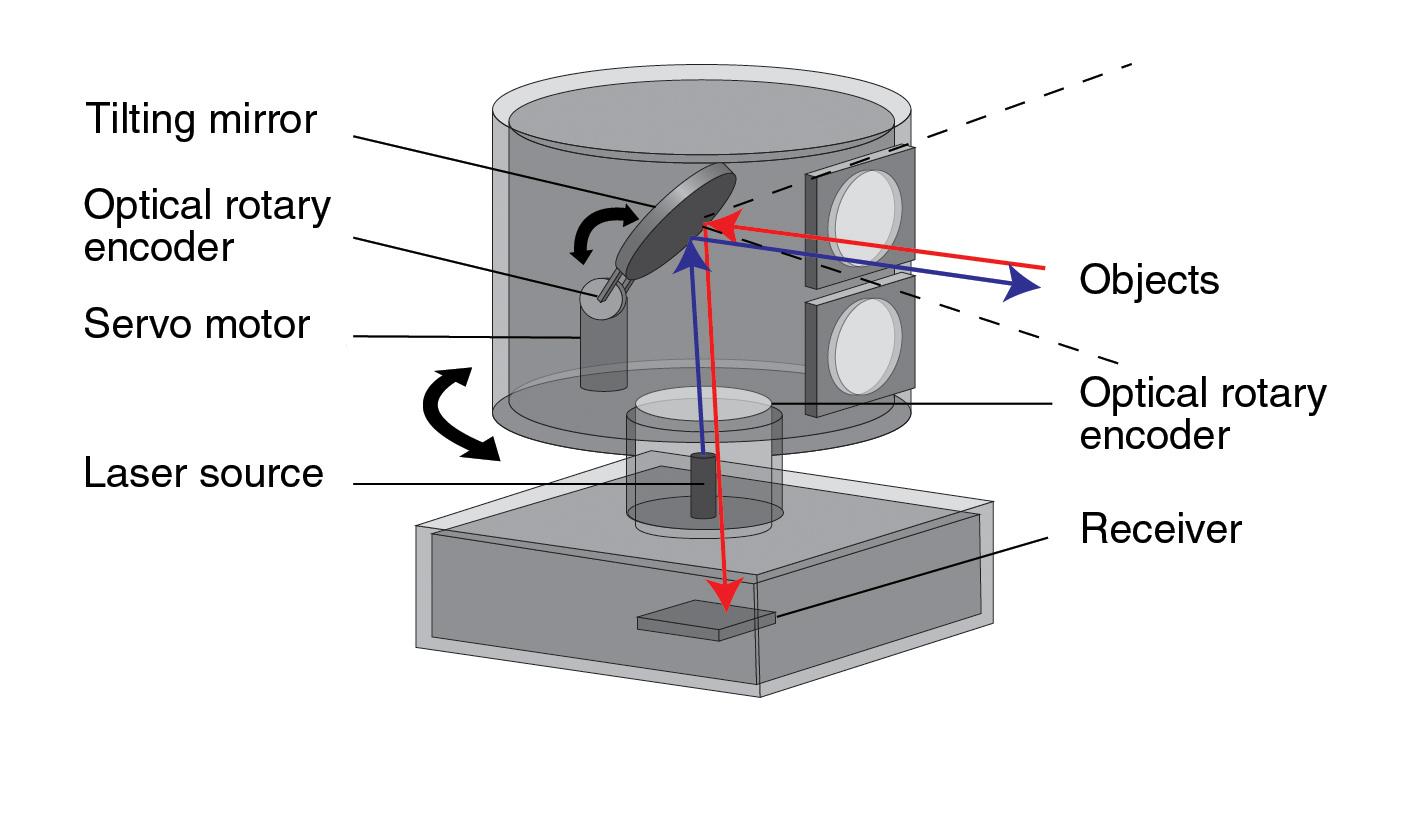
\includegraphics[scale=1]{img/lidar.jpg}
  \caption{Example of a LiDAR scanner.}
  \label{fig:lidar}
\end{figure}


\subsection{LiDAR scanner and context}
\label{subsc:lidar}
LiDAR\footnote{This paragraph is inspired by \cite{lidar}.} is an acronym of Light Detection and Ranging. It is a remote sensing technology which uses the pulse from a laser to collect measurements. The principle is simple: it works in a similar way to Radar and Sonar but uses light waves from a laser, instead of radio or sound waves. A LiDAR system calculates how long it takes for the light to hit an object or surface and reflect back to the scanner and then, uses the velocity of light\footnote{The velocity, or speed of light is 299,792,458 metres
per second.} to calculate the distance. LiDAR systems can fire around 1,000,000 pulses per second.

When scanning, there are two kind of rotations that a LiDAR scanner performs. They are indicated by black arrows in Figure~\ref{fig:lidar}. Not only a LiDAR scanner has a constant rotation angle when turning on itself but it also has a constant vertical rotation angle when scanning the environment. Because of these constant rotation angles, the further we go, the lower the point density is. On the contrary, the closer to the scanner we are, the higher the point density is. This density variation can be observed in
Figure~\ref{fig:density}. To conclude, extracting the most dense areas is interesting as they always are around scanner locations and then, reduce the global search area.

\begin{figure}
  \centering
  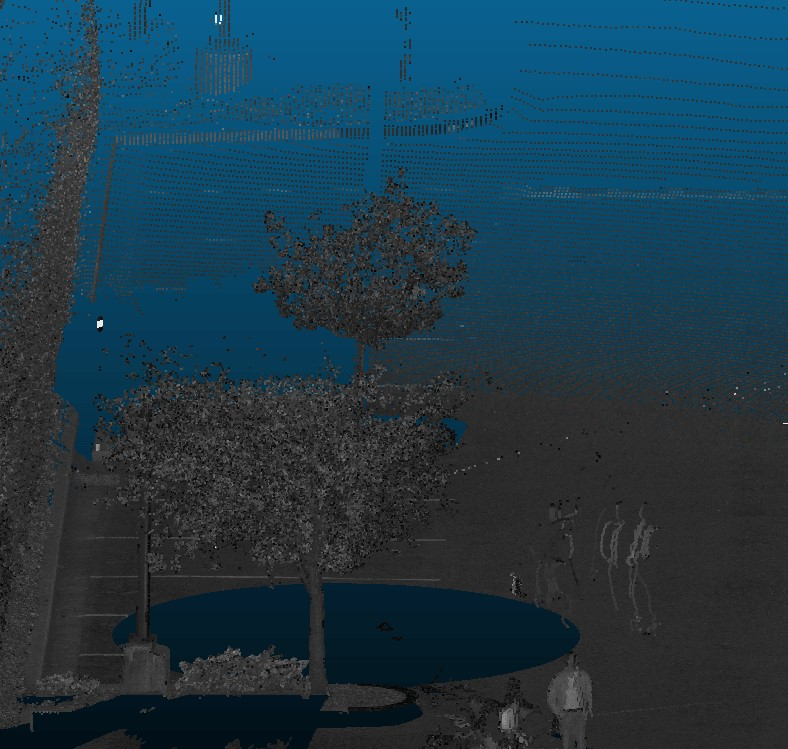
\includegraphics[scale=0.7]{img/dens.jpg}
  \caption{Variation of density as we go further away from the scanner source (the empty circular space).}
  \label{fig:density}
\end{figure}


\subsection{Clustering and dense area extraction}
\label{subsc:highdens}
\begin{figure}
  \centering
  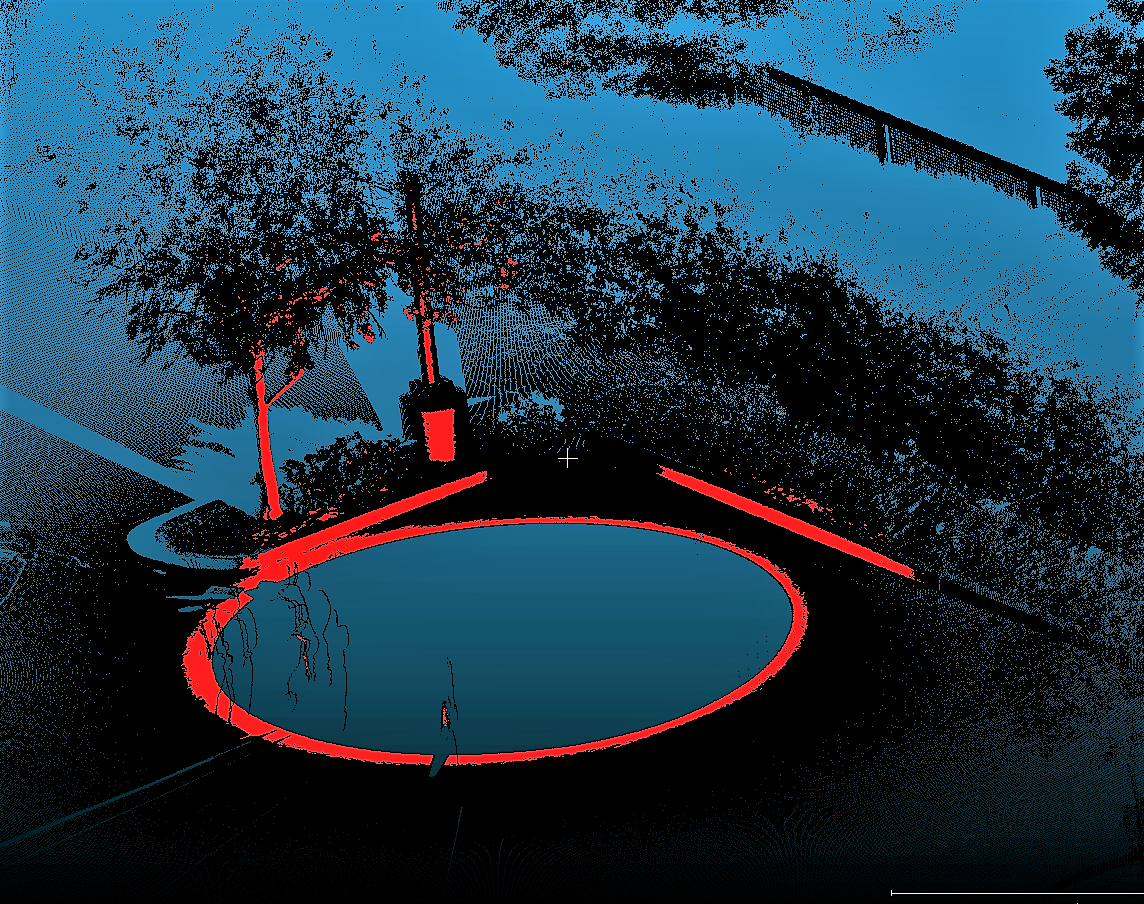
\includegraphics[scale=0.44]{img/highdens.png}
  \caption{The result of the high density extraction of a point cloud.}
  \label{fig:highdens}
\end{figure}

\begin{figure}
  \centering
  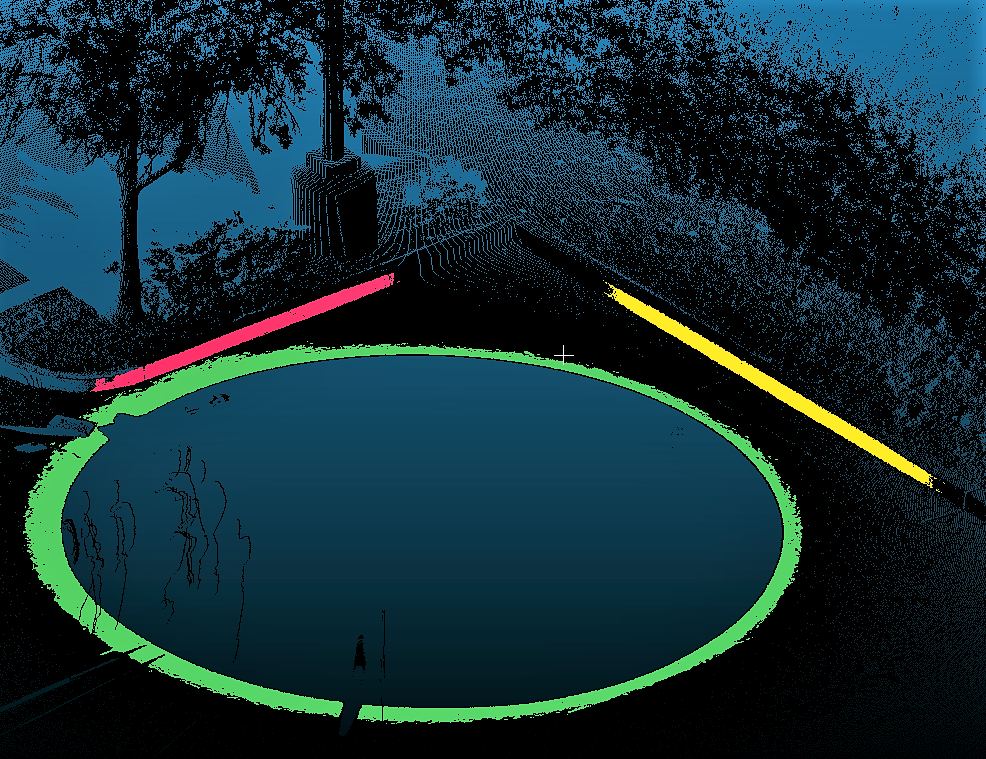
\includegraphics[scale=0.5]{img/cluster.png}
  \caption{The result after clustering dense points of Figure~\ref{fig:highdens}.}
  \label{fig:cluster}
\end{figure}

\begin{figure}
  \centering
  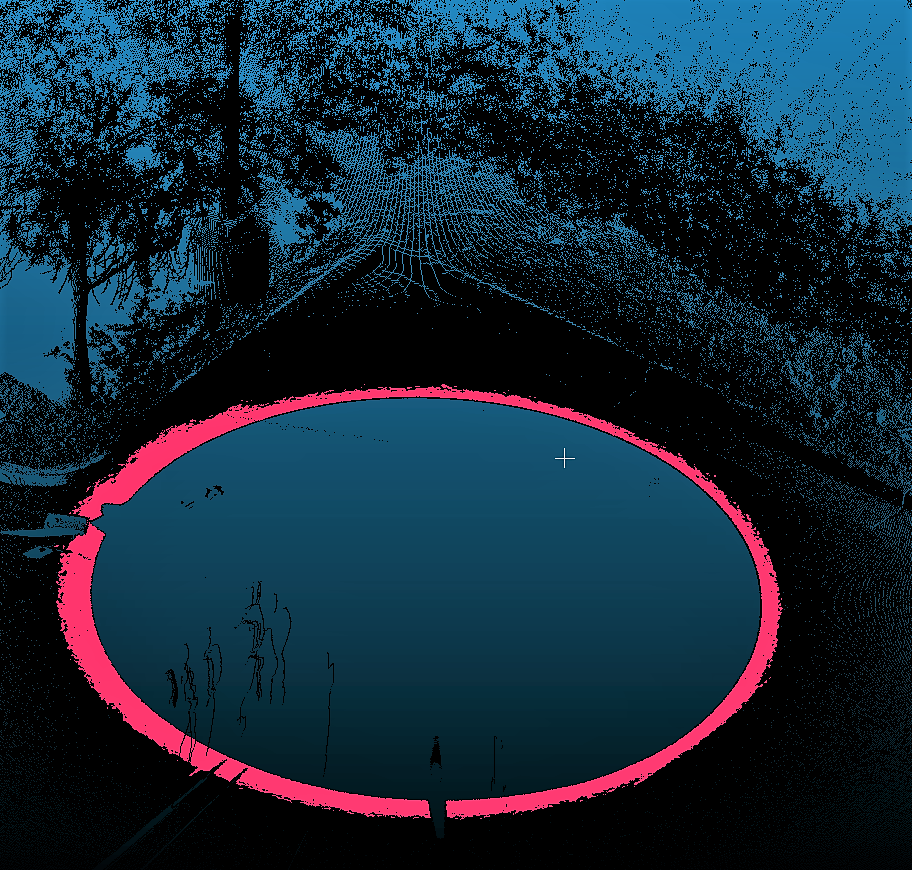
\includegraphics[scale=0.5]{img/circular.png}
  \caption{The result after trying to identify circular clusters of Figure~\ref{fig:cluster}.}
  \label{fig:circular}
\end{figure}

The first step of the algorithm is to detect high density regions in the point cloud. For each point, we compute its density based on the mean distance to its $k$ neighbors ($k \in [15,50]$). We extract high density regions by selecting a percentage of the densest points (percentage between 1 and 5\%). Figure~\ref{fig:highdens} shows some results of this high density point extraction. As you can see, they always are around the scanner's location. Note that the scanner is not able to scan below
himself leading to an elliptic empty form\footnote{This elliptic form is the key point of the method described in Section~\ref{sc:elliptic}.} appearing in all point clouds.

Once these points are extracted, a clustering step is applied. The clustering is needed so that points from the point clouds corresponding to potentially different parts of the scene around the scanner can be separated. For each point, we compute its non-oriented normal and the associated \emph{confidence level} by performing a principal component analysis (PCA) on its local neighborhood. Section~\ref{subsc:pca} gives more details on how this PCA works. Then, as long as points are not attributed
to a cluster, we select the point on the flattest surface, and iteratively add its neighbors that share a coherent normal orientation (the dot product of the two normals must be superior to 0.8 in our experiments). Note that the  flattest surface is determined using condifence levels, they tell which point belongs to a planar region. Figure~\ref{fig:cluster} shows the result of such clustering.

Once every point is clustered, we discard clusters with too few points (in our experiments, we use a threshold of 0.2\% of the number of high density points). We then detect clusters that are circular. A cluster is considered circular if its centroid, i.e. the average of all the points it contains, is far away from the points of the cluster. Figure~\ref{fig:circular} shows a circular cluster identified.

At this point, we have computed a rough estimate of the scanner's location. Methods described in Section~\ref{sc:grid-pattern} and Section~\ref{sc:elliptic} use it in their own way in order to find scanner locations.



\section{The grid-pattern method}
\label{sc:grid-pattern}
This section explains one approach we tried in order to solve the problem. Before explaining the method in detail, let us first give the intuition behind this idea.

\subsection{Intuition}
As said in Section~\ref{subsc:lidar}, LiDAR scanners perfom two kind of rotations. These constant vertical and horizontal rotation angles reveal some grid patterns on surfaces perpendicular to the ground\footnote{To be precise, perpendicular to the surface on which the scanner is installed.}. Figure~\ref{fig:grid1} shows an example of a grid pattern that can be found in point clouds. The purpose here is to find, for a single grid pattern, a relation between all constant rotation angles and the scanner's position. Therefore, this relation can be applied with all possible grid patterns in the point clouds, leading to a problem with a huge set of
constraints to solve. The idea is that only the real scanner's location is able to explain in the best way these constant rotation angles.

\begin{figure}[h]
  \centering
  
\includegraphics[scale=0.5]{img/grid1.png}
  \caption{Example of a grid pattern. As you can see there is a constant offset between each vertical line and each horizontal lines. Note that the offset between columns is not necessary the same than between lines.}
  \label{fig:grid1}
\end{figure}

This algorithm can be divided into two parts. The first step is to find \emph{accurate} grid patterns in point clouds. Once this is done, the second step is to build the equation that will be solved. These two parts are explained in the following subsections. Note that this approach does not work in multiscan mode, compare to the other approach described in Section~\ref{sc:elliptic}. It assumes there is only one scanner which explains all grid-patterns in the point cloud.

\subsection{Grid-pattern matching}
This subsection explains how to find \emph{accurate} grid patterns in point clouds in order to reduce as much as possible the noise and its impact during the problem resolution described in Section~\ref{subsc:eq}. A set of point is considered as an \emph{accurate} grid-pattern when:
\begin{itemize}
  \item it is planar as much as possible\footnote{Because of the noise.},
  \item the underlying planar surface is orthogonal to the surface of the ground,
  \item the gap between columns is consistent enough,
  \item the gap between lines is consistent enough.
\end{itemize}


\begin{algorithm}[tb]
  \SetAlgoVlined
  \DontPrintSemicolon
  \SetKw{Report}{report}
  \SetArgSty{}
  \SetKwFunction{GetPlanarPatches}{GetPlanarPatches}
  \SetKwProg{Fn}{Function}{}{}
  \Fn{\GetPlanarPatches{P}}{
    \KwIn{a pointcloud $P = \left\lbrace p_i \mid i \in [0, s]  \right\rbrace$.}
    \KwOut{a set of potential grid-pattern patches.}
    \tcc{We compute the normal of each point and keep both confidence level and normal $\left\langle \mu_i, \vec{v}_i \right\rangle$.}
    \tcc{See Section~\ref{subsc:pca} for more details on PCA algorithm.}
    \tcc{From here, $\forall i \in [0, s]$ we assume $\vec{v}_i$ to be the normal at $i$ and $\mu_i$ its confidence level.}
    \For{$i = 0;\ i < s;\ i = i + 1$}{
      $\left\langle \mu_i, \vec{v}_i \right\rangle \gets PCA($50 closest neighbours of $i)$\;
    }
    $R\gets\emptyset$\;
    visited $\gets\emptyset$\;
    \For{$i = 0;\ i < s;\ i = i + 1$}{
      \tcc{ Continue if already visited or is not planar enough.}
      \If{$i \in$ visited or $\mu_i > 0.001$}
      {\Continue}
      tmp $\gets \left\lbrace p_i \right\rbrace$\;
      \ForEach{$j \in $ 50 closest neighbours of $i$}{
        \tcc{If $\vec{v}_j$ and $\vec{v}_i$ are almost colinear and $j$ has not been seen yet.}
        \If{abs($\vec{v}_j \times \vec{v}_i$) $> 0.9$ and $j \not\in$ visited}{
          tmp $\gets$ tmp $\cup\ p_j$\;
          visited $\gets$ visited $\cup\ j$\;
        }
      }
      \tcc{If there is enough point for a grid-pattern patch.}
      \If{size of tmp $> 0.9\ \times$ 200}{
        $R \gets R\ \cup $ tmp
      }
    }
    \Return{$R$}\;
  }
  \caption{Find various not-overlaping planar patches in a point cloud.
    \label{alg:GetPlanarPatches}}
\end{algorithm}

Algorithm~\ref{alg:GetPlanarPatches} shows how to extract some planar patches in a point cloud. A preprocessing step already done and explained in Section~\ref{subsc:highdens} is to compute for each point of the point cloud, the normal and its \emph{confidence level}. This \emph{confidence level} plays a key role in the algorithm as it tells how planar the region around each point is. By browsing all points, each time we find a point with a good \emph{confidence level} ($> 0.001$), we start to build a patch around it. To do so, we extract its 50
closest neighbours and consider only those having their normal almost colinear to the normal of the starting point. If the size of the obtained set is bigger enough ($>\ 0.9 \times 200$), the set is kept and otherwise, not. Also, in order to avoid overlaping or patches too close, we keep track of visited points.

Although planar, this set of patches potentially contains: \textbf{(a)} patches whose underlying surfaces are not orthogonal to the surface of the ground and \textbf{(b)} patches without grid patterns. To filter out each \textbf{(a)} patch, we use a dot product between its normal and the normal of the circular cluster found in the high-density area\footnote{The circular cluster desribes the surface on which the scanner is positioned.} (see Section~\ref{sc:highdens}). For \textbf{(b)} patches,
the objectif is to indentify grid-patterns. To do so, we use least square method in order to fit lines. Least-square is explained in Section~\ref{subsc:least}. Fitting a line fall into linear least square problems. Figure~\ref{fig:fitline} shows how to fit a line to a set of points using the Eigen library~\cite{eigenweb}. The purpose is to use this line fitting in order to cluster lines and columns. Figure~\ref{fig:line-col-cluster} shows results of a clustering performed on two patches after several fittings and adjustements. We only keep firstly patches containing a grid-pattern and then, patches having a regular gap between columns and lines. The rest is discarded.

\begin{figure}
  \centering
  \begin{lstlisting}
    Eigen::VectorXf FitLine(std::vector<A3D::Point_3dPlus> const& points)
    {
      Eigen::MatrixXf mat(points.size(), 2);
      Eigen::VectorXf vec(points.size());
      int count = 0;
      for (auto it = points.begin(); it != points.end(); ++it)
      {
        mat(count, 0) = static_cast<float>(it->x());
        mat(count, 1) = static_cast<float>(it->y());
        vec(count++) = 1.0;
      }
      return mat.fullPivHouseholderQr().solve(vec);
    }
  \end{lstlisting}
  \caption{Function using least-square to fit a line to the given set of points.}
  \label{fig:fitline}
\end{figure}

\begin{figure*}[t!]
  \centering
    \begin{subfigure}[t]{0.5\textwidth}
      \centering
        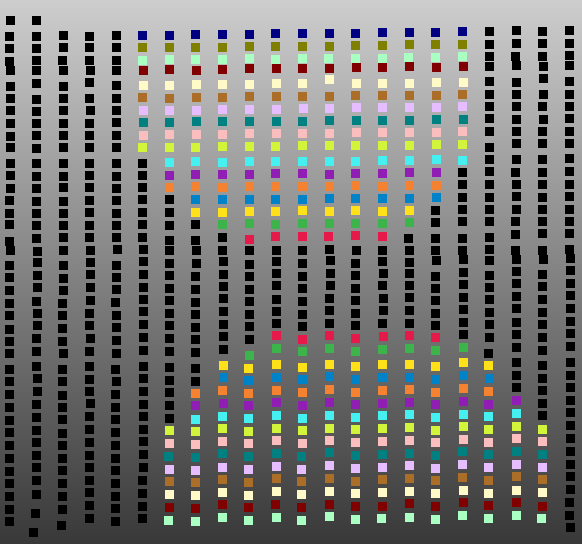
\includegraphics[height=2.5in]{img/grid-lines.png}
        \caption{Lines clustering performed on two patch.}
    \end{subfigure}%
    ~
    \begin{subfigure}[t]{0.5\textwidth}
      \centering
        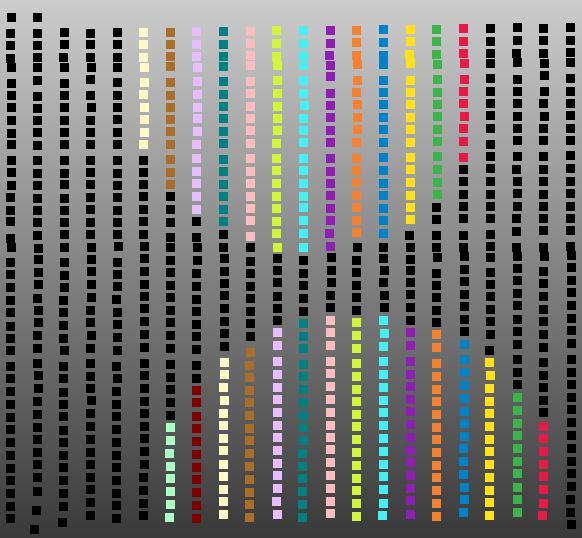
\includegraphics[height=2.5in]{img/grid-cols.png}
        \caption{Column clustering performed on two patches.}
    \end{subfigure}
    \caption{Example of columns and lines clustering in order to identify grid-patterns.}
    \label{fig:line-col-cluster}
\end{figure*}

Once only \emph{accurate} patches are kept, columns and lines are identified, the problem can be formalised.

\subsection{Equation to solve}
\label{subsc:eq}

For a little recall of Section~\ref{sc:grid-pattern}, the purpose here is to find a relation between the scanner's position (what we are looking for) and the regular gaps between lines and columns. At this point, we already have a reduced area of research which is around the circular cluster obtained in Section~\ref{subsc:highdens}. What we need, is a set of constraints that will help to set the scanner at a specific position within this area.

Look at Figure~\ref{fig:topview}. There are four (4) vertical lines viewed from a bird's eye: $a$, $b$, $c$ and $d$. They are represented as points because of the point of view. A regular between them can be observed. As explained in the introduction to LiDAR scanners (Section~\ref{subsc:lidar}) this regular gap is due to the consistent angle of rotation of the scanner $\alpha_1 = \alpha_2 = \alpha_3$.

These angles directly involve the scanner location in all equations. Here is how the problem is built: each time the scanner location is set, we minimize for each grid-pattern, and for each pair of two consecutive lines (or columns), the absolute difference between their respective angles. In our case me minimize:
\begin{align*}
  d_1 &= |\alpha_1 - \alpha_2|\\
  d_2 &= |\alpha_2 - \alpha_3|\\
\end{align*}

This is a non-linear least-square problem which can be resolved using the Ceres Solver~\cite{ceres} (Section~\ref{subsc:least}).

\begin{figure}
  \centering
  \begin{tikzpicture}
    \draw[fill] (0,0) circle (2pt) coordinate (a) node[above=0.2cm]{$a$};
    \draw[fill] (2.5,0) circle (2pt) coordinate (b) node[above=0.2cm]{$b$};
    \draw[fill] (5,0) circle (2pt) coordinate (c) node[above=0.2cm]{$c$};
    \draw[fill] (7.5,0) circle (2pt) coordinate (d) node[above=0.2cm]{$d$};
    \draw[fill] (3.75, -4.5) circle (2pt) coordinate (e) node[below=0.1cm,black]{$s$};
    \draw[dashed] (a) -- (e) -- (b)
      pic["$\alpha_1$", draw=red, red, solid, <-, angle eccentricity=1.2,
          angle radius=1cm] {angle=b--e--a};
    \draw[dashed] (b) -- (e) -- (c)
      pic["$\alpha_2$", draw=red, red, solid, <-, angle eccentricity=1.2,
          angle radius=1.2cm] {angle=c--e--b};
    \draw[dashed] (c) -- (e) -- (d)
      pic["$\alpha_3$", draw=red, red, solid, <-, angle eccentricity=1.2,
          angle radius=1.4cm] {angle=d--e--c};
  \end{tikzpicture}
  \caption{A top view over four (4) vertical grid lines ($a$, $b$, $c$ and $d$) and a scanner ($s$).}
  \label{fig:topview}
\end{figure}

\subsection{Results and discussions}
\begin{figure}
  \centering
  \begin{tikzpicture}
    \draw[fill] (0,0) circle (2pt) coordinate (a) node[above=0.2cm]{$a$};
    \draw[fill] (2.5,0) circle (2pt) coordinate (b) node[above=0.2cm]{$b$};
    \draw[fill] (5,0) circle (2pt) coordinate (c) node[above=0.2cm]{$c$};
    \draw[fill] (7.5,0) circle (2pt) coordinate (d) node[above=0.2cm]{$d$};
    \draw[fill] (3.75, -4.5) circle (2pt) coordinate (e) node[below=0.1cm,black]{$s$};
    \draw[fill] (-4, 0) circle (2pt) coordinate (f) node[below=0.1cm,black]{$s'$};

    \draw[dashed] (a) -- (e) -- (b)
      pic["$\alpha_1$", draw=red, red, solid, <-, angle eccentricity=1.2,
          angle radius=1cm] {angle=b--e--a};
    \draw[dashed] (b) -- (e) -- (c)
      pic["$\alpha_2$", draw=red, red, solid, <-, angle eccentricity=1.2,
          angle radius=1.2cm] {angle=c--e--b};
    \draw[dashed] (c) -- (e) -- (d)
      pic["$\alpha_3$", draw=red, red, solid, <-, angle eccentricity=1.2,
          angle radius=1.4cm] {angle=d--e--c};

    \draw[dashed, blue] (a) -- (f) -- (b)
      pic["$\alpha_1'$", draw=blue, blue, above, solid, <-, angle eccentricity=1.2,
          angle radius=1cm] {angle=b--f--a};
    \draw[dashed, blue] (c) -- (f) -- (d)
      pic["$\alpha_2'$", draw=blue, blue, below, solid, <-, angle eccentricity=1.2,
          angle radius=1cm] {angle=d--f--c};

  \end{tikzpicture}
  \caption{Illustration of the problem preventing the grid-pattern method from finding the scanner location. Note that this is a top view over four (4) vertical grid lines ($a$, $b$, $c$ and $d$), the apprixmation ($s'$) and the real scanner ($s$).}
  \label{fig:grid-problem}
\end{figure}

\begin{figure}[h]
  \centering
  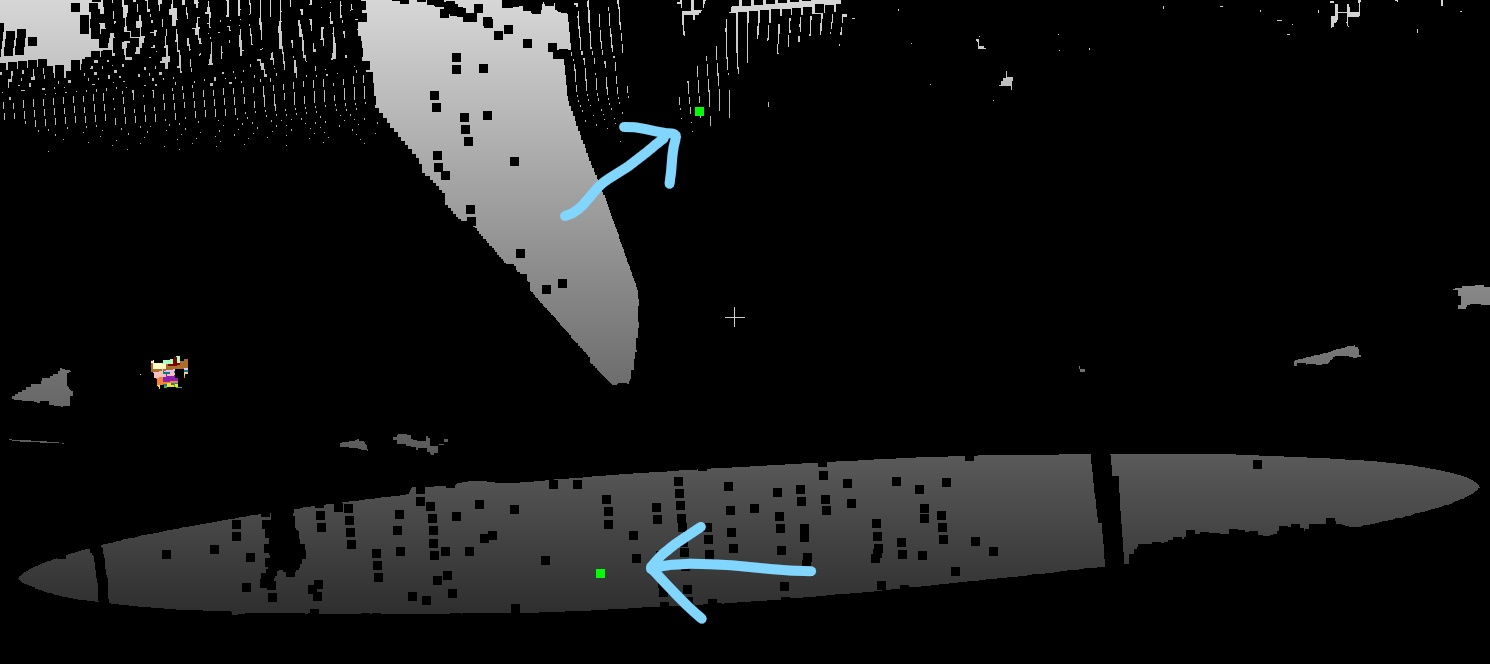
\includegraphics[scale=0.3]{img/grid-result.jpg}
  \caption{An approximation of the scanner location using the grid-pattern method. The real scanner location is highlighted by the upper arrow while the approximation is highlighted by the lower one.}
  \label{fig:grid-result}
\end{figure}

Figure~\ref{fig:grid-result} shows a result of grid-pattern approximation of scanner location. This method does not perform quite well. One would think that the approximation is not far from the real scanner location but reducing the area of research to a cube around the circular cluster can be misleading. We tried to remove the area constraints and observed that the approximation moves entirely away from the real location and even the point cloud itself. It can stoop pretty low, go to really
high altitude, on the left, on the right. It completely depends on the distribution of the grid-patterns in the point cloud.

Let us take one grid-pattern in order to illustrate the problem: Figure~\ref{fig:grid-problem}. As our method tries to minimize the differences between all pairs of angles, here $\alpha_1$, $\alpha_2$ and $\alpha_3$, the ideal case is if the scanner location belongs to the underlying surface of the grid-pattern in which case:
\begin{align*}
  |\alpha_1 - \alpha_2| &= 0\\
  |\alpha_2 - \alpha_3| &= 0\\
\end{align*}

Therefore, with a huge set of equations involving several grid-patterns, the optimal solution for
the solver is to put the scanner on the \emph{mean plan of all grid-pattern's underlying planes}. This is why, without the reduced area constraint, the approximated scanner is far away from the point cloud as the solver tries to reduce all angle differences and then, satisfy all grid-patterns. Another problem found is that this method is too much subjected to noise. We are talking about really small values for angle differences that we want to minimize. A small noise can have
huge effects during the solving.

To conclude, angles differences are not discriminating enough. We believe there is a way to express the problem, in order to bypass this behaviour but we deciced to try another approach presented in Section~\ref{sc:elliptic}. The current approach is limited to one scanner whereas the other one works with multiple scaners, therefore, is more interesting for \CC.


\section{The elliptic method}
\label{sc:elliptic}
This section describes the second approach to solve the scanner location finding problem. This approach is more interesting than the one of Section~\ref{sc:grid-pattern} because it works natively with merged point clouds (multiple scanners within a point cloud). Let us have the intuition of this method.

\subsection{Intuition}
Let us remind that a first common step to both methods which finds circular clusters is performed. It is described in Section~\ref{sc:highdens}. This first step finds all circular areas around all scanners locations.


\subsection{Fitting ellipse}
\begin{figure}[h]
  \centering
  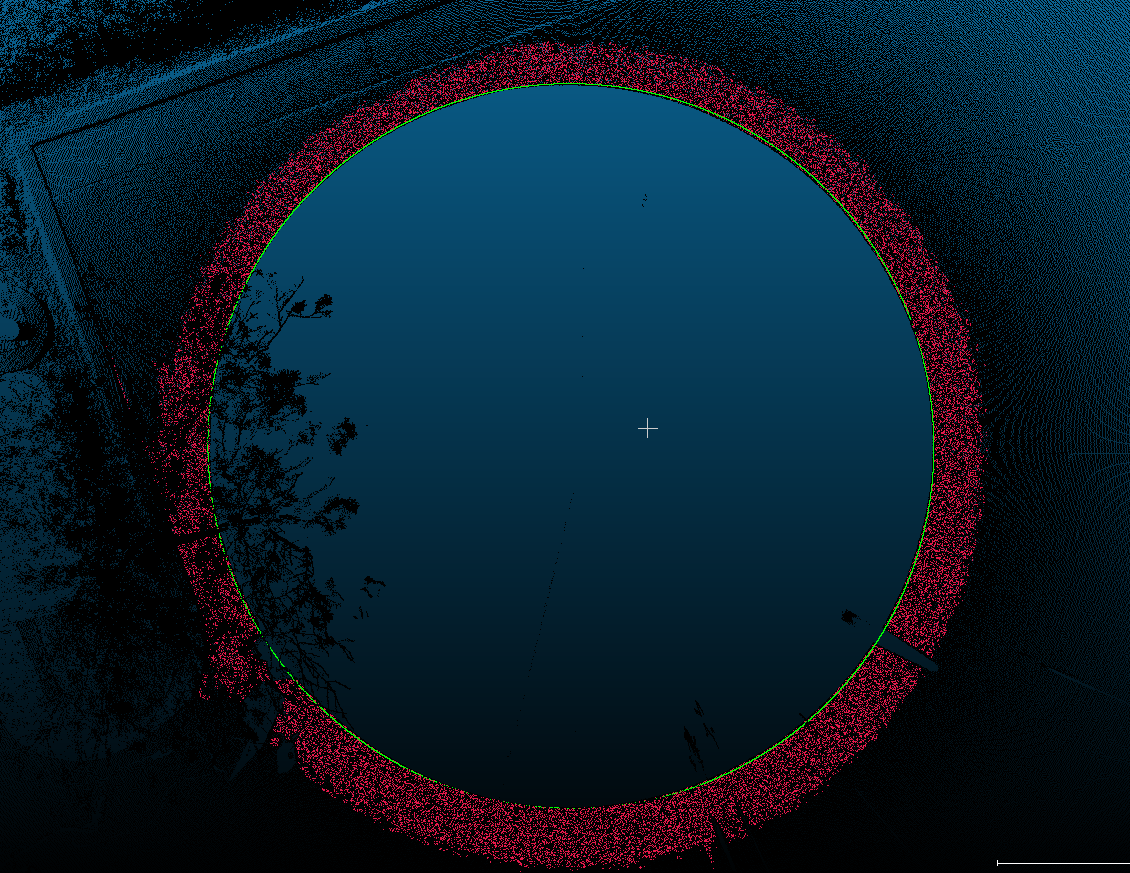
\includegraphics[scale=0.4]{img/ellipse.png}
  \caption{Ellipse fitted on a circular cluster.}
  \label{fig:ellipse}
\end{figure}

For each of the circular cluster, we extract the points close to the inside of the cluster and then fit an ellipse using a least-square algorithm.

FIXME: Explain ellipse fitting (refere to ransac and least square in background).

The center of the fitted ellipse is computed, and the center of the scanner lies on the z-axis passing through this center. This is only an approximation that suppose that the ground is approximately horizontal. This approximation applies to a vast majority of cases where terrestrial scanning is used. If needed, a refinement of the horizontal position of the scanner can be obtained by applying the same process as described below to estimate the vertical position of the scanner.

\subsection{Equation to solve}
To estimate the height of the scanner, we will use the slight variation in density of the points in the circular cluster. The intuition is that the density of a local point is linked to its distance from the scanner. Using multiple points, we are able to triangulate the position of the scanner. For a point $p$ in the high density circular cluster, we note $r$ the distance between the scanner and the point, $d$ the density of the point, and $\alpha$ the angle between the normal of the point and the direction
from the point of the scanner. Using the fact that point density decreases proportionally as moving away from the scanner, the following relation should be verified for any pair of points.
\begin{equation}
\frac{d_a \times r_a^2}{\cos(\alpha_a)} = \frac{d_b \times r_b^2}{\cos(\alpha_b)}
\end{equation}
where $d_a$ is the density of $a$ and $d_b$ the density of $b$. This is explained in Figure~\ref{fig:sideview}.

For each circular cluster, we pick a sample of N points (in our experiments, N=6 points) with different densities. We then use a non-linear least square solver to determine the position of the scanner, mixing together   equations (15 if N=6). As a result, we retrieve an estimated position of the scanner location.

\begin{figure}
  \centering
  \begin{tikzpicture}[scale=0.8]
    \draw[fill] (-8.2,0) circle (0pt) coordinate (p1);
    \draw[fill] (6.5,0) circle (0pt) coordinate (p2);
    \draw[gray, thin] (p1) -- node[near end, right=3cm]{ground level} (p2);

    \draw[fill] (0,0) circle (0pt) coordinate (x) node[above=0.2cm]{};
    \draw[fill] (5,0) circle (0pt) coordinate (y) node[above=0.2cm]{};
    \draw[fill,blue] (5.5,0) circle (2pt) coordinate (a) node[below=0.2cm]{$a$};
    \draw[fill,red] (-2,0) circle (2pt) coordinate (b) node[below=0.2cm]{$b$};
    \draw[fill] (5.5,2) circle (0pt) coordinate (c);
    \draw[fill] (-2,2) circle (0pt) coordinate (d);
    \draw[black, dashed, <->, line width=0.5mm] (x) -- node[below=-0.1cm]{ellipse} (y);
    \draw[blue](a) circle [radius=4.05];
    \draw[red](b) circle [radius=5.2];
    \draw[fill] (2.45,2.7) circle (4pt) coordinate (s) node[right=0.2cm]{$s$};
    \draw[dashed, blue] (s) -- node[near start, right]{$r_a$} (a) -- (c)
      pic["$\alpha_a$", draw=blue, blue, solid, <-, angle eccentricity=0.8,
          angle radius=1cm] {angle=c--a--s};
    \draw[dashed, red] (d) -- (b) --  node[near end, left=0.1cm]{$r_b$} (s)
      pic["$\alpha_b$", draw=red, red, solid, <-, angle eccentricity=0.8,
          angle radius=1cm] {angle=s--b--d};
    \draw[red, <-, line width=0.3mm] (d) -- node[left, near start]{$\vec{n}_b$}(b);
    \draw[blue, <-, line width=0.3mm] (c) -- node[right, near start]{$\vec{n}_a$}(a);
  \end{tikzpicture}
  \caption{A side view of the ellipse and two spheres intersecting at the scanner position $s$ and their respective centers $a$ and $b$. We have the relation $\frac{d_a \times r_a^2}{\cos(\alpha_a)} = \frac{d_b \times r_b^2}{\cos(\alpha_b)}$ where $d_a$ is the density of $a$ and $d_b$ the density of $b$.}
  \label{fig:sideview}
\end{figure}


\subsection{Results and discussions}
\begin{figure}[h]
  \centering
  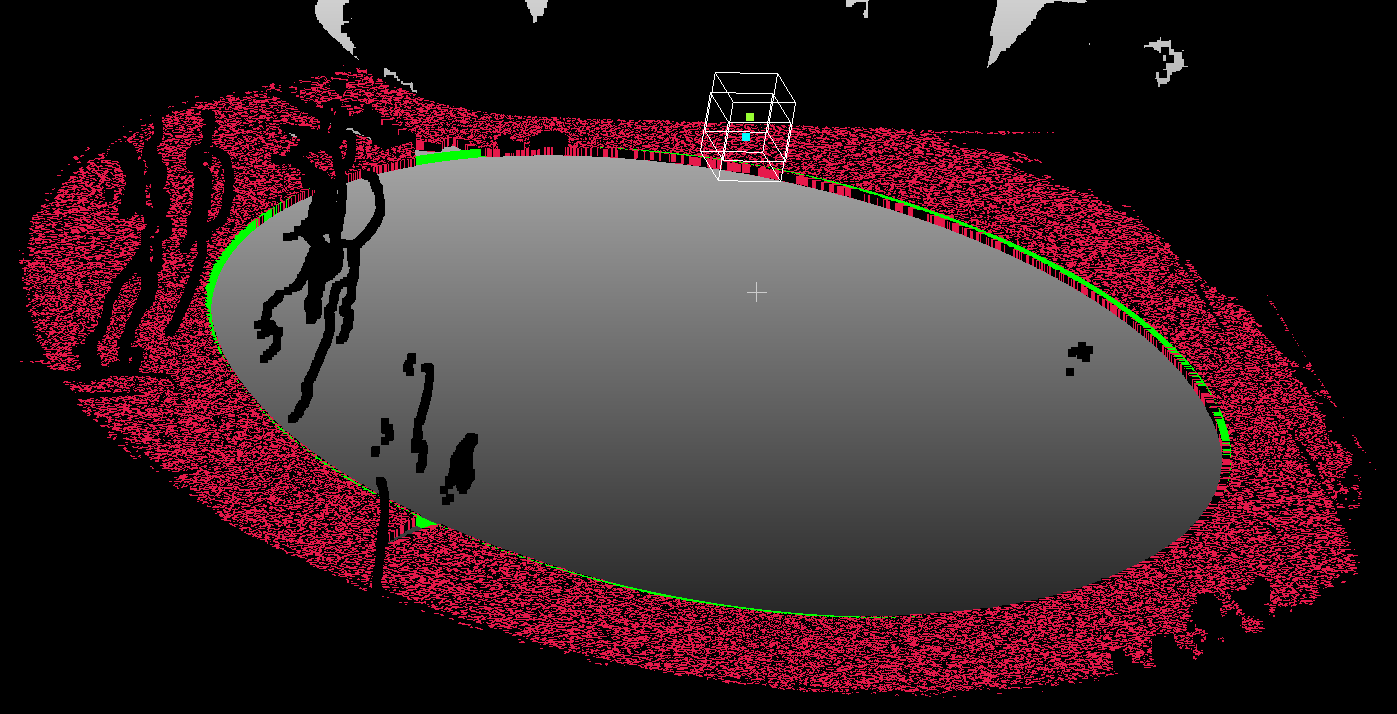
\includegraphics[scale=0.4]{img/ellipse-result.png}
  \caption{Light blue point in the box is the correct position, green point next to it is our estimation.}
  \label{fig:ellipse-result}
\end{figure}
\begin{figure}[h]
  \centering
  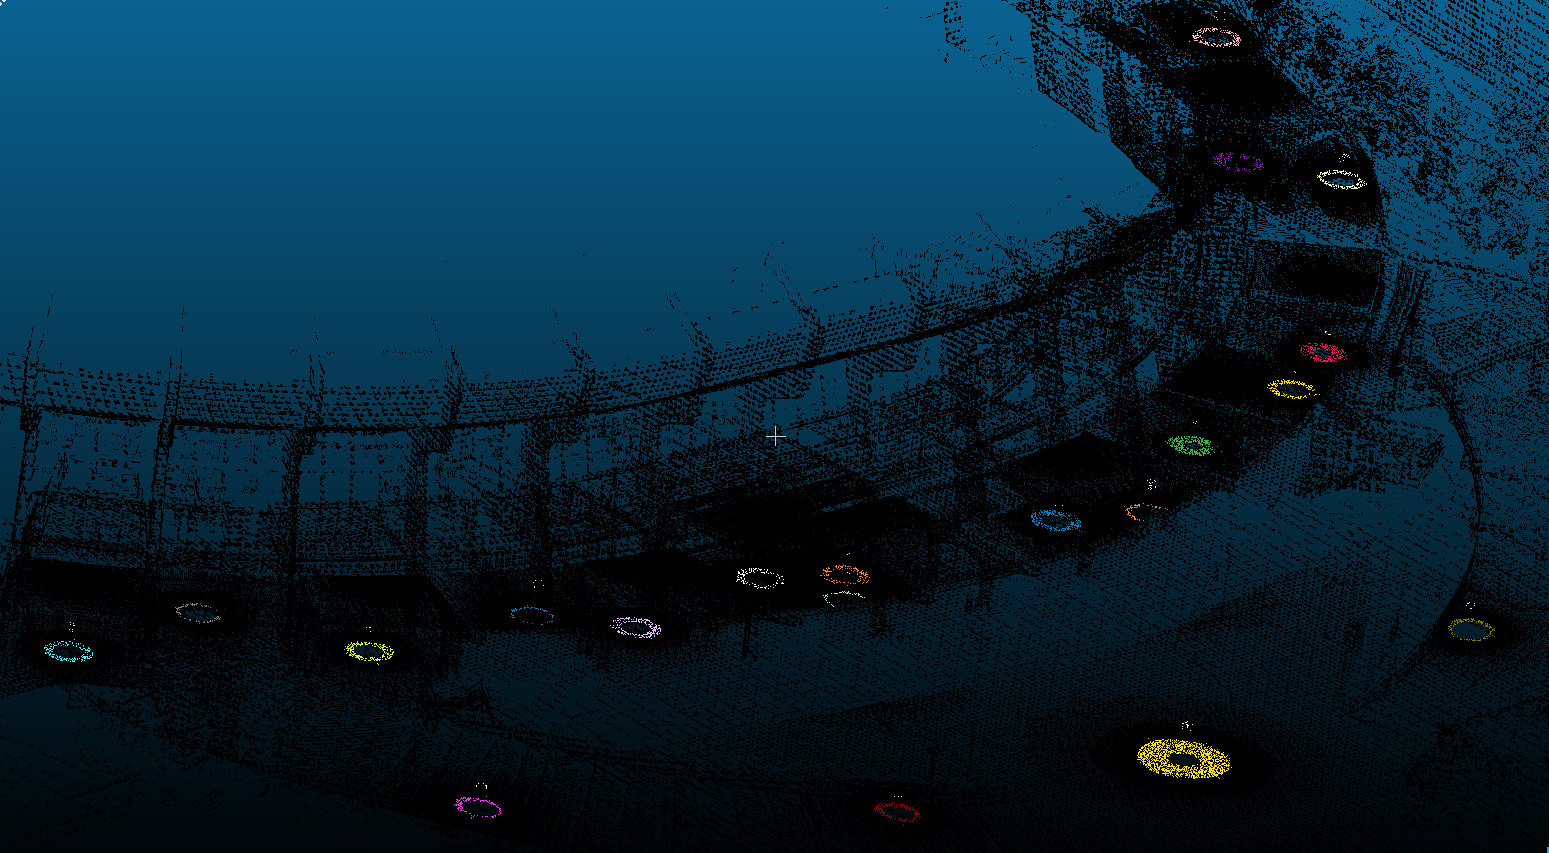
\includegraphics[scale=0.3]{img/ellipse-multi1.png}
  \caption{Multiple locations detected in a large point cloud.}
  \label{fig:ellipse-multi1}
\end{figure}
\begin{figure}[h]
  \centering
  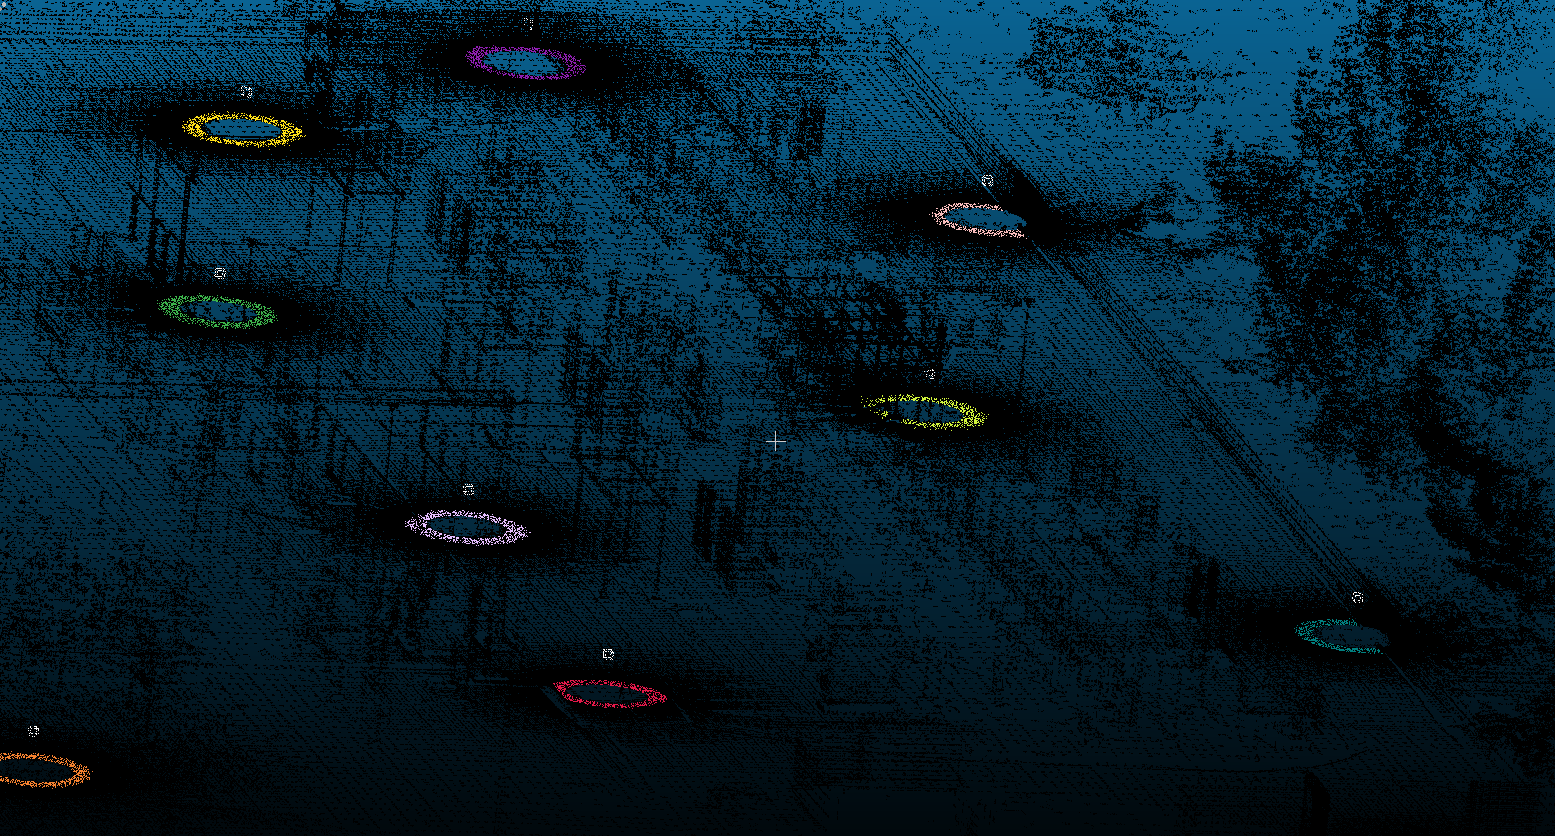
\includegraphics[scale=0.3]{img/ellipse-multi2.png}
  \caption{Multiple locations detected in another large point cloud.}
  \label{fig:ellipse-multi2}
\end{figure}

Testing on various reference datasets, we found that the error between the correct position and our estimation ranges between 2 and 20 cm.

This pipeline is particularly suited for multi-scan point clouds. Terrestrial scanners tend to generate most of the points close to their positions. If we consider that scans are not taken in the same close vicinity, high density clusters are disjoint. We confirm with hypothesis in our experiments. Therefore, the coarse detection works well in the multi-scan hypothesis. The same idea applies for the fine position algorithm: most points in the circular cluster come from a single scanner. The few other points coming from different scanners don’t have a significant impact on the local density of the points. That way, the scanner height is correctly detected in a multi-scan setting.

\chapter{Point Cloud Visibility}
\label{ch:visibility}
This chapter introduces our custom point cloud visibility algorithm. It starts by giving in Section~\ref{sc:spec-visibility}, a clear context for the presented work. Then, Section~\ref{sc:related-visibility} gives an overview of the previous related work and describes some experimentations of a previously-published point cloud visibility algorithm. Finally, as nothing seems to be well adjusted for our specific case we implemented a custom point cloud visibility algorithm described in Section~\ref{sc:custom}.

\section{Specifications}
\label{sc:spec-visibility}

\subsection{Context}
Currently in \CC, there is a way to still use a point cloud for reconstructing purposes even if the scanner's location information is lost. It gives the user the opportunity to manually set the scanners position on a 3D representation of the point cloud. But, only one position can be set. It requires that the point cloud contains points resulting from \emph{one and only one} scanner\footnote{Also known as monoscan point cloud.}. This is because, during the reconstruction, \CC uses
the scanner location to orient the normals at each point. In a monoscan point cloud case, it simply orients each normal toward the scanner. But in case of multiscan point cloud, it needs to know for each point, toward which scanner the normal must be oriented, which is less simple to find.

Therefore, even if \emph{ScanFinder} (Chapter~\ref{ch:scanfinder}) is applied on a LAS format\footnote{A point cloud format that \CC wants to support and which does not store scanner locations in its metadata.} multiscan point cloud in order to retrieve all scanner positions, the reconstruction is still infeasible for \CC. This is where a point cloud visibility algorithm is useful in order to attribute each point to a scanner. Have in mind that a point can be seen by two scanners, especially if there is no physical barrier between them. In this case it is difficult to exactly know which scanner produced the point. But, as this point-scanner attribution is only required for normal orientations, we only need to know which scanner best sees it.

\subsection{Objective}
As a final step toward supporting point clouds without scanner locations, the algorithm must:
\begin{itemize}
\item take as input any 3D point cloud captured from static scanners as well as the location of all scanners,
\item be invariant to differences between scanners, such as: density, noise, rotation angle,
\item find for each point the scanner which best sees it, not necessary the scanner which produced it,
\item have a reasonnable running time.
\end{itemize}

As for \emph{ScanFinder} described in Chapter~\ref{ch:scanfinder}, the algorithm is not expected to work with mobile point clouds.


\section{Related work}
\label{sc:related-visibility}
This section highlight some previous work on the subject of \emph{Point cloud visibility} before describing in detail one approach that we tried and the results obtained.

\subsection{Previous work}
Visibility in point clouds is a sucessful topic that experienced several publications since the 1960s~\cite{appel, sutherland, funkhouser, greene, bittner}.

\subsection{An interesting approach: Visibility of Noisy Point Cloud Data}
\label{subsc:noisy}

\subsubsection{Intuition}

\subsubsection{The algorithm}

\subsubsection{Results and discussions}


\section{A custom disk-based approach}
\label{sc:custom}

\subsection{Overview}


\subsection{Implementation}


\subsection{Results and discussions}

\chapter{Point Cloud Compression}
\label{ch:compression}
This Chapter present the last subject of the internship, \emph{point cloud compression}. Section~\ref{sc:spec-compression} gives a lead on the context bringing such need. Then, Section~\ref{sc:work-compression} mentions notable previously-published work on the subject. In Section~\ref{sc:custom-compression} we describe a custom arithmetic approach. The benchmark result highlights the relevance of Zip Compression to our objectives. Finally, Section~\ref{sc:integration}
discusses \emph{Zip compression} integration to \CC.

\section{Specifications}
\label{sc:spec-compression}

\subsection{Context}
As said in the introduction, \CC provides a cloud service for client not having performant machines. When a client submit a job, at some point, data uploading starts including the point cloud (if available\footnote{The reconstruction can also be made with photos.}). If the upload fails due to lost internet connection or any other reason, the upload restarts from scratch. Many point clouds are huge with a file size over $10$ GB, some of them more than $100$ GB. A Point cloud
easily becomes the biggest part of the data being upload to the cloud service. Therefore, reducing its size before uploading it, is a first good step toward better cloud services. This is where the scope of this work ends. A second step would probably be to find a way to send data through streaming with a recovery system on the cloud in case of fail.

This is how the need for \emph{Point Cloud Compression} emerged.

\subsection{Objective}
The method of compression must observe the following rules:
\begin{itemize}
  \item take as input any point cloud, provided it is static.
  \item being lossless,
  \item being able to compress several fields such as: point locations, normals, colors, intensity,
  \item compress the point cloud size ideally by two (2),
  \item have a reasonable compressing time such that the uploading time saved thanks to file size reduction is not lost during point cloud compression.
\end{itemize}

\section{Related work}
\label{sc:work-compression}
This section introduces different approach for point cloud compression. There is a need for clarification. The term \emph{point cloud compression} generally refers to ingenious representations of point clouds such that they take less space and can be easily loaded and used. However, for easy readability purposes we also use \emph{point cloud compression} to refer to simple arithmetic compression even if they are applied without no context of what is being compressed.

\cite{qsplat, schnabel, gumhold, zhang}. // FIXME\\
\cite{brotli, 7zip}

Dire que les compressions arithmétiques ont l'avantage de pouvoir compresser sans se soucier du décompressement, utilisation facile, optimisations géométriques...

\section{A bit-wise compression of point cloud}
\label{sc:custom-compression}
This section describes a custom point cloud compression. It is not exaclty a compression algorithm as it is just a packed representation of the same point cloud.It just ignores useless data reguardind the needed precision. Section~\ref{subsc:overview-packed} explains how this packed representation is obtained while Section~\ref{subsc:compression-benchmark} compares it with Brotli, 7Z (LZMA) and Zip, other arithmetic compression algorithms.

\subsection{Overview}
\label{subsc:overview-packed}


\subsection{Comparison with Brotli, 7Z and Zip}
\label{subsc:compression-benchmark}

\begin{sidewaysfigure}[t]
    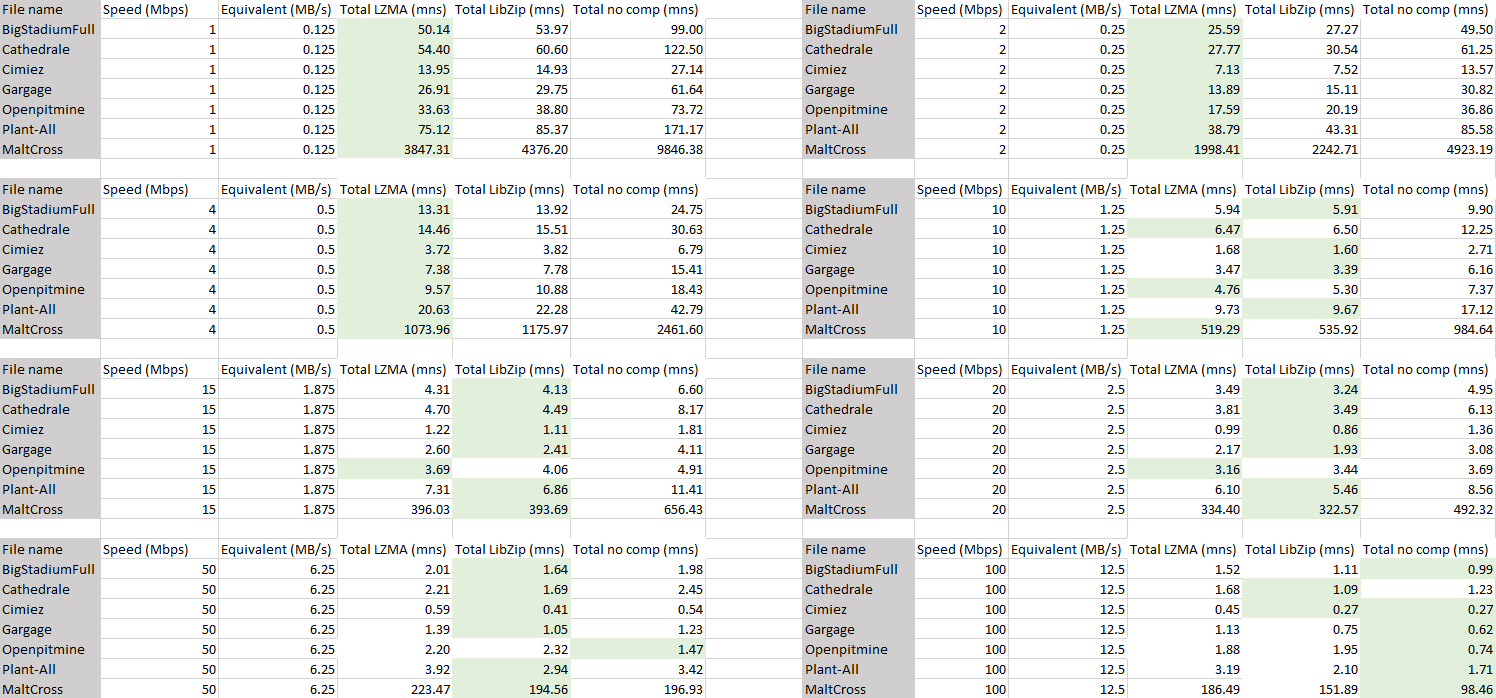
\includegraphics[width=\textwidth]{img/compare1.png}
    \caption{Caption in landscape to a figure in landscape.}
    \label{fig:compare-excel}
\end{sidewaysfigure}


\section{Integration of Zip compression}
\label{sc:integration}

\subsection{Code interface}
\begin{figure}
  \centering
  \begin{lstlisting}
  namespace Zip
  {
      bool compress(std::string const& inputPath, std::string const& outputPath,
              zip_progress_callback pf = nullptr, void* pProgressData = nullptr);

      bool decompress(std::string const& inputPath, std::string const& outputPath);
  }
  \end{lstlisting}
  \caption{Function using least-square to fit a line to the given set of points.}
  \label{fig:fitline}
\end{figure}


\subsection{\CC Software}


\chapter{Conclusion}
\label{ch:conclusion}

\section{Summary of Internship Achievements}

Summary.


\section{Applications}

Applications.


\section{Future Work}

Future Work.


\appendix
% appendices come here


\addcontentsline{toc}{chapter}{Bibliography}
\bibliographystyle{alpha}
\bibliography{bib/references}

\end{document}
